\documentclass[11pt]{article}
\usepackage[T1]{fontenc}
\usepackage{lmodern,amsmath,amssymb,booktabs,tabularx,graphicx,microtype,pdflscape}
\usepackage[letterpaper,margin=0.8in]{geometry}
\usepackage[hidelinks]{hyperref}
\usepackage{fancyhdr}
\pagestyle{fancy}\fancyhf{}\fancyhead[L]{\small Width and precision in constructive MLPs}\fancyhead[R]{\small Section 3 research note 5}\fancyfoot[C]{\thepage}
\setlength{\headheight}{14pt}
\setlength{\emergencystretch}{2em}
\allowdisplaybreaks[2]
\begin{document}
\begin{center}
{\Large What the method-comparison table does not show}\\[4pt]
{\normalsize Error versus network size at fixed arithmetic precision}\\[6pt]
{\small Section 3 research note 5 --- 25 September 2026}
\end{center}
\vspace{0.5em}

The comparison table gives QUILL and ChebNet the same logarithmic order of width in the requested accuracy. It does not tell us how many neurons either method actually needs, where finite precision stops further improvement, or whether a larger network remains useful at the available precision. The recent tapout comparisons measure these differences directly. We retain the experiment's label \emph{QUILLS} for QUILL in the figures and tables below.

The main observation is a tradeoff. QUILLS reaches the beginning of its low-error plateau with fewer total hidden neurons. ChebNet generally reaches a lower final error on the three harder targets, but uses more neurons and several hidden layers to do so. The staircase and Costarelli--Spigler curves are still decreasing with size when the budget ends; their remaining error barely changes as arithmetic precision increases. The tested Mhaskar construction instead gains little from additional size at these precisions. A single asymptotic rate or a single final-error entry does not show these distinct behaviors.

Figures 1--2 contain the error-versus-neuron curves, with the original four precision rows split across two pages for readability. They use the existing data, with no new constructions or training. This is an empirical comparison of the implemented methods and searched candidates, not a lower bound on what any architecture could achieve.

\section{What is being compared}

The four targets, all on \([-1,1]\), are
\[
e^x,\qquad \sin(4\pi x),\qquad \frac{1}{1+25x^2},\qquad
\sin\!\bigl(8\pi(x+1)^2\bigr).
\]
Each panel fixes the target and the arithmetic precision \(p\), counted in significant binary digits. Its horizontal axis is the allowed number \(N\) of \emph{total hidden neurons}, summed over layers. Thus QUILLS counts its one hidden layer, including halo neurons; ChebNet counts all of its hidden layers. The paper's table instead reports \emph{maximum layer width}. The figure's size unit is deliberate and must not be confused with that table column or with the number of parameters.

For a method \(A\), let \(\mathcal C_{A,p}\) be its tested networks at precision \(p\). For a candidate \(g\), let \(n(g)\) be its total hidden-neuron count and \(e_{\mathrm{val}}(g)\) its relative \(L^2\) error on the validation grid. We plot
\[
E_A(N,p)=\min_{\substack{g\in\mathcal C_{A,p}\\n(g)\le N}}e_{\mathrm{val}}(g),
\qquad
e_{\mathrm{val}}(g)=
\left(\frac{\sum_{x\in X_{\mathrm{val}}}|g(\operatorname{round}_p x)-f(x)|^2}
{\sum_{x\in X_{\mathrm{val}}}|f(x)|^2}\right)^{1/2}.
\tag{1}
\]
Here \(X_{\mathrm{val}}\) contains 1021 uniformly spaced cell midpoints. The network receives the rounded input, while the error is measured against the target at the exact grid point. These are validation-selection curves, not independent reporting-grid errors. The best-so-far definition makes every curve nonincreasing in \(N\); a flat segment can mean that the same smaller candidate remains best.

We evaluate (1) on the cap grid \(\mathcal G=\{\operatorname{round}(32\cdot2^{k/4}):k=0,\ldots,20\}\), from 32 to 1024 with four points per doubling. The full precision sweep is \(p=9,11,\ldots,51,53\); the figures show \(21,33,45,53\). The last row uses native binary64 for QUILLS and ChebNet, as specified in Appendix A. No wall-clock or construction-cost comparison is implied.

\section{What the curves add}

\paragraph{The number of neurons needed before improvement slows.}
Reading left to right at a fixed precision, QUILLS makes its steep decrease earlier than ChebNet on sine, Runge, and the chirp. To mark the beginning of the low-error region consistently, define
\[
E_A^*(p)=E_A(1024,p),\qquad
N_A^*(p)=\min\{N\in\mathcal G:E_A(N,p)\le 10E_A^*(p)\}.
\tag{2}
\]
The large circles mark this \emph{tapout width} when the comparison's qualification checks allow it. The factor ten means ``within one decimal order of the best observed error under the cap,'' not that the network has stopped improving exactly. If the marker occurs at 32, all we know is \(N_A^*\le32\) at the resolution tested. Appendix A explains when a curve is classified as still limited by width instead.

Across the 17 tested precisions from 21 to 53 bits, ChebNet's tapout width is about 2.0--3.4 times QUILLS' for sine, 4.0--5.7 times for Runge, and 1.7--2.4 times for the chirp. On \(e^x\), QUILLS is already in this region by the smallest tested width; ChebNet needs at most 64 neurons. These are finite-grid comparisons, not fitted asymptotic constants.

\paragraph{How low the final error gets.}
Reading downward at a fixed size, the QUILLS and ChebNet plateaus move down as more bits become available. Their best errors are approximately a target- and implementation-dependent multiple of the unit roundoff \(2^{-p}\). ChebNet's best error is lower on the three harder targets: the paired median advantages over the tested \(p\ge21\) are 3.8 bits for sine, 2.4 for Runge, and 4.5 for the chirp. QUILLS' median floor is slightly lower on \(e^x\), although ChebNet is lower at the native-FP64 endpoint.

The native-FP64 values illustrate both sides of the tradeoff:
\begin{center}\small
\begin{tabular}{lrrrr}
\toprule
&\multicolumn{2}{c}{Tapout neuron cap \(N_A^*\)}&\multicolumn{2}{c}{Best error under 1024 neurons \(E_A^*\)}\\
Target & QUILLS & ChebNet & QUILLS & ChebNet\\
\midrule
\(e^x\)&\(\le32\)&64&\(1.99\times10^{-15}\)&\(2.66\times10^{-16}\)\\
\(\sin(4\pi x)\)&91&181&\(6.74\times10^{-15}\)&\(1.19\times10^{-15}\)\\
Runge&152&861&\(1.87\times10^{-14}\)&\(8.97\times10^{-16}\)\\
Chirp&304&512&\(1.04\times10^{-13}\)&\(5.06\times10^{-15}\)\\
\bottomrule
\end{tabular}
\end{center}
The two error columns are the best values under the full cap; they are not the errors at the marked tapout widths. For example, the Runge result says that QUILLS enters its near-floor region much earlier, while ChebNet eventually attains about twenty times smaller error. Neither fact cancels the other.

\paragraph{Why the other methods stop improving.}
The staircase and Costarelli--Spigler curves nearly overlap across the higher-precision rows, but still slope downward as neurons are added. Their limiting resource in this range is size, not additional bits. At \(p=53\) and the 1024-neuron cap, their errors range from approximately \(2\times10^{-6}\) to \(9\times10^{-3}\), depending on target and method. The flat Mhaskar curves have a different meaning: larger candidates fail to improve on smaller ones at the available precision. Its best native-equivalent 53-bit error is about \(5\times10^{-12}\) on \(e^x\), \(2.3\times10^{-2}\) on Runge, and of order one on sine and the chirp. The latter two therefore have no tapout marker. A marker on its Runge curve does not indicate high precision; equation (2) only measures proximity to that method's own best error.

\paragraph{Comparing the same error, rather than each method's own plateau.}
A tapout comparison alone is not a matched-accuracy comparison, because ChebNet's plateau is lower. At each tested odd precision from 15 through 53, the smallest \emph{plotted neuron cap} at which QUILLS reaches an error threshold in the nonempty interval \([4E_{\mathrm{QUILLS}}^*(p),\,0.1]\) is no larger than ChebNet's. The original check used 80 thresholds per interval; checking every attained-error breakpoint gives the same ordering on \(\mathcal G\). This is a comparison at the grid's resolution: two different actual neuron counts can fall under the same cap. Closer to QUILLS' best error, even the cap ordering need not hold.

\clearpage
\begin{landscape}
\thispagestyle{plain}
\begin{figure}[p]\centering
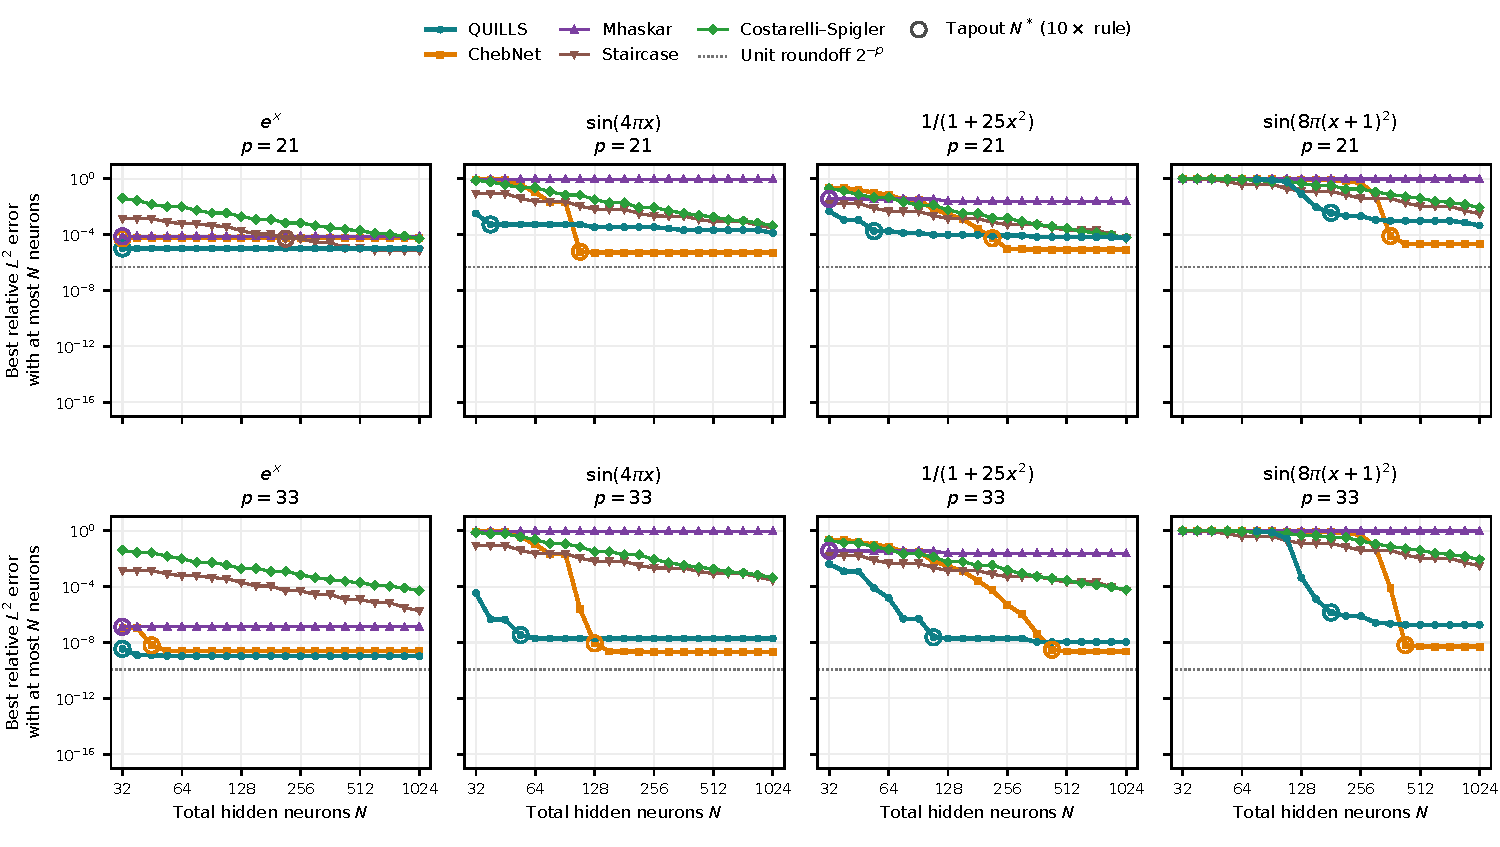
\includegraphics[width=\linewidth]{figures/tapout_curves_p21_p33.pdf}
\caption{Error versus allowed total hidden neurons, at \(p=21\) and \(p=33\). Columns are the four targets; each curve is the smallest validation error among that method's tested candidates using at most the stated number of neurons. The dotted line is unit roundoff, not a guaranteed error floor. Large circles mark the qualified \(10\times\) tapout criterion in (2). QUILLS begins its low-error plateau at smaller sizes; ChebNet usually reaches a lower plateau on the harder targets. The staircase and Costarelli--Spigler curves continue decreasing with size. All panels have the same axis limits.}
\end{figure}
\end{landscape}
\clearpage
\begin{landscape}
\thispagestyle{plain}
\begin{figure}[p]\centering
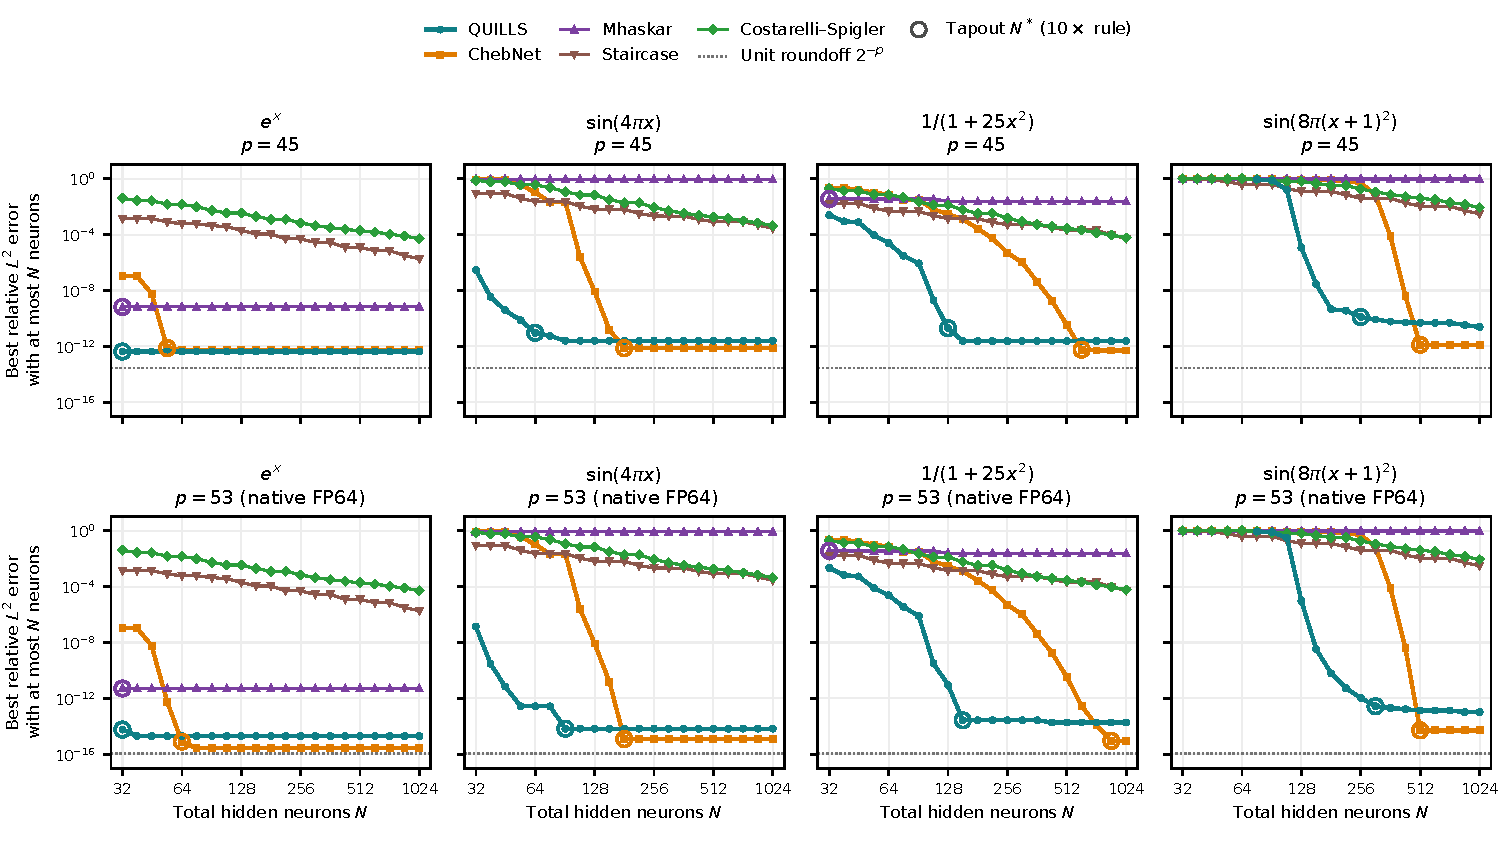
\includegraphics[width=\linewidth]{figures/tapout_curves_p45_p53.pdf}
\caption{The same saved comparison at \(p=45\) and native FP64 (\(p=53\)). More bits move the QUILLS and ChebNet plateaus downward; they have little effect on the width-limited staircase and Costarelli--Spigler curves. The Mhaskar envelope remains flat because larger tested candidates do not beat the smaller candidates. These panels, together with Figure 1, reproduce the original \(4\times4\) curve grid in a larger, readable format. The FP64 row uses the native arithmetic paths described in Appendix A and is not a continuation with identical operation order.}
\end{figure}
\end{landscape}
\clearpage\appendix
\section{Protocol and interpretation of the comparison}

\subsection{Arithmetic and measurement}
For \(p\le51\), construction and inference use the \texttt{pfloat} format \((p,-958,959)\), with round-to-nearest, ties-to-even arithmetic. Every model addition, multiplication, division, and square root is rounded at \(p\) bits. The tanh implementation is also evaluated using these operations; least squares uses the statement-by-statement \(p\)-bit port of LAPACK \texttt{DGELSS}. No high-precision readout solve is inserted into a low-precision model. Constants and target-oracle answers are rounded once before entering the model. Each method may choose its own sample locations and sample count; target access is of the same type, not the same sampling budget.

The \(p=53\) QUILLS endpoint uses NumPy tanh and SciPy \texttt{gelsd}, with cutoff \(2^{-52}\). ChebNet uses a native binary64 discrete cosine transform for its Chebyshev coefficients and a NumPy forward pass. Both native paths use NumPy target evaluations, native exponents, and matrix products whose summation order differs from the sequential \(p\)-bit implementation. The other three methods retain their 53-bit sweep results. These paths all have 53 significant bits, but the last precision increment does not isolate a change in bit count alone.

The validation grid has 1021 midpoints. An earlier 1024-point midpoint grid aligned with some staircase jump locations and understated its error; that grid was replaced. The current code and data use 1021, even though the older specification text still states 1024. The separate reporting grid has 8001 points. The curves in this note use validation error because they compare all candidates under each size cap; the original fixed-budget experiment's reporting-grid curves are a different result. Residual norms are evaluated with a 320-bit error meter against higher-precision target values. This meter only reads the model output and does not improve the construction or inference arithmetic.

\subsection{Candidate constructions and size coverage}
QUILLS uses uniform tanh centers with halo \(H=\min(24,\lfloor W/4\rfloor)\), where \(W\) is its total hidden width, and interior spacing \(h=2/(W-2H-1)\). The slope is \(\gamma=\lambda/h\), with \(\lambda\) chosen by the existing bandwidth rule at tolerance \(2^{1-p}\). The readout is solved from 4801 target samples. At \(p\le51\), its candidates cover every plotted grid width through 512, plus the earlier sweep's widths 96, 192, 384, 768, and 1024. In particular, widths 609, 724, and 861 were not constructed for QUILLS at those precisions; their plotted values are the best available smaller candidate. This missing coverage can only worsen its best-error envelope. The native-FP64 comparison includes every plotted width.

ChebNet realizes a Chebyshev expansion as a deep ReQU network, using 4096 nodes for coefficient formation, a pruned hierarchical construction, and optional power-of-two coefficient normalization. Its 52 candidate degrees range from 1 to 250 under the 1024-total-neuron cap. The tanh methods use a single hidden layer. Mhaskar converts a polynomial approximation into finite differences of tanh features; the displayed curve includes the better-conditioned common-grid variant tested in expC13, not only the original separate stencils. The staircase includes validated steepness, midpoint-jump, and extrapolated-halo options. Costarelli--Spigler includes the tested centered-sample and truncation options. Thus these curves compare the best implemented candidates offered to each method, rather than one unoptimized textbook formula per method.

The other three methods reuse their existing candidate sweeps. Mhaskar's degree grid stops at 128, giving a largest tested candidate of 257 neurons; the staircase and Costarelli--Spigler candidates extend to the 1024-neuron cap. The flat Mhaskar envelope above 257 is therefore also a consequence of candidate coverage, not a measurement of newly constructed larger networks. Its 32-neuron tapout marker is not necessarily its best candidate's actual size: the best 53-bit Runge candidate has 113 neurons. The earlier 3073-parameter experiment is not the budget applied to ChebNet in this figure.

\begin{samepage}
For context, the selected native-FP64 networks at the tapout caps have:
\begin{center}\small
\begin{tabular}{lrrrrr}
\toprule
&\multicolumn{2}{c}{QUILLS}&\multicolumn{3}{c}{ChebNet}\\
Target&Total neurons&Layers&Total neurons&Maximum width&Layers\\
\midrule
\(e^x\)&32&1&62&30&4\\
\(\sin(4\pi x)\)&91&1&178&82&6\\
Runge&152&1&786&386&8\\
Chirp&304&1&496&242&7\\
\bottomrule
\end{tabular}
\end{center}
\end{samepage}
Layers count hidden layers; QUILLS' maximum width equals its total neurons. A selected network may have fewer neurons than its plotted cap. ChebNet's maximum individual layer is smaller than QUILLS' width on three of these four selected pairs, despite its larger total neuron count. This is why the figure's conclusion must name the size measure. Neither measure gives construction time: the figure does not compare the cost of a least-squares solve with the cost of polynomial coefficient formation and network construction.

\subsection{How much the tapout definition matters}
The plotted best value \(E_A^*\) is only the minimum over tested candidates under a finite cap. We call it a precision floor when increased precision reduces it while additional size offers little improvement. The plotting routine withholds a tapout marker if the error exceeds 0.1. It classifies a useful fit as width-limited when two additional bits improve the cap error by less than a factor of two, while increasing the neuron cap from 724 to 1024 still improves error by at least a factor of 1.5. At \(p=53\), the unavailable 53-to-55 comparison is replaced by the 51-to-53 comparison. These are empirical classifications, not certified limiting-error statements.

The factor ten was chosen to mark where the steep decline begins to flatten. It matters because QUILLS often continues improving slowly after this point. A stricter factor-two rule can reverse an ordering: on the chirp at \(p=21\), QUILLS' threshold moves from the 181-neuron cap to 861, whereas ChebNet's moves from 362 to 431. This corrects the earlier report's overly narrow summary of that sensitivity. The common-error comparison in Section 2 avoids comparing different multiples of different methods' floors, but still uses the plotted cap grid. For example, at \(p=21\) and sine error \(4E^*_{\mathrm{QUILLS}}\approx5.27\times10^{-4}\), QUILLS uses 108 neurons and ChebNet uses 96; both fall under the plotted cap of 108. The grid-based result must not be strengthened into an exact neuron-count dominance claim.

\section{Sources and checks for this note}
The tapout comparison was reviewed by Sam on 25 September 2026. This note uses that comparison, not the separate draft sweep extending to 128 bits. Its source files are:
\begin{itemize}\raggedright
\item The current paper supplied for the appendix sweep, Table 1, stored as \path{docs/appendix_materials/2026-09-25/supplied/current_paper.pdf}.
\item \path{results/checkpoint_C_geometry/expC13_five_method_comparison/expC13_results.md} and the same folder's \path{data/tapout.json}, \path{data/tradeoff_rows.jsonl}, and \path{data/candidates/}.
\item \path{experiments/expC13_five_method_comparison/tapout_plot.py}, \path{tradeoff_plot.py}, \path{tradeoff_data.py}, \path{common.py}, and \path{SPEC.md}.
\end{itemize}
All 20 target/method error envelopes were reconstructed from the saved candidates, and their derived tapout records agree exactly with the saved \texttt{tapout.json}. The width ratios, paired floor differences, selected FP64 model sizes, grid-based common-error comparison, and threshold sensitivity were independently checked. No new model evaluation or training was performed.
\end{document}
